\chapter{Cài đặt môi trường và chương trình}
\section*{I. BACKEND}

\section{Cài đặt Python}

Python là ngôn ngữ lập trình cốt lõi cho dự án Django của chúng ta. Django 5.0.13 yêu cầu Python phiên bản 3.10 trở lên.

\subsection{Bước 1: Tải và cài đặt Python}

\begin{enumerate}
    \item Truy cập trang web chính thức của Python tại \url{https://www.python.org/downloads/}
    \item Tải phiên bản Python phù hợp (khuyến nghị Python 3.10 hoặc cao hơn)
    \item Trong quá trình cài đặt, đảm bảo tích vào tùy chọn "Add Python to PATH"
\end{enumerate}

\begin{tcolorbox}[colback=yellow!10, colframe=yellow!50!black, title=Lưu ý quan trọng]
Đối với người dùng Windows, việc thêm Python vào biến môi trường PATH là rất quan trọng để có thể chạy Python từ Command Prompt hoặc PowerShell.
\end{tcolorbox}

\subsection{Bước 2: Xác nhận cài đặt thành công}

Mở Command Prompt (Windows) hoặc Terminal (macOS/Linux) và chạy lệnh:

\begin{lstlisting}[language=bash]
python --version
\end{lstlisting}

hoặc

\begin{lstlisting}[language=bash]
python3 --version
\end{lstlisting}

% \begin{figure}[H]
%     \centering
%     \includegraphics[width=0.7\linewidth]{python_version.png}
%     \caption{Kết quả lệnh kiểm tra phiên bản Python}
%     \label{fig:python-version}
% \end{figure}

\section{Cài đặt MongoDB}

MongoDB là cơ sở dữ liệu NoSQL được sử dụng trong dự án của chúng ta để lưu trữ dữ liệu.

\subsection{Bước 1: Tải và cài đặt MongoDB}

\begin{enumerate}
    \item Truy cập trang web chính thức của MongoDB: \url{https://www.mongodb.com/try/download/community}
    \item Tải phiên bản MongoDB Community Edition phù hợp với hệ điều hành của bạn
    \item Tiến hành cài đặt theo hướng dẫn của trình cài đặt
    \item Đối với Windows, chọn "Complete" trong quá trình cài đặt để cài đặt MongoDB Compass (giao diện đồ họa)
\end{enumerate}

\subsection{Bước 2: Khởi động MongoDB}

\subsubsection{Windows}
MongoDB thường được cài đặt như một dịch vụ và tự khởi động. Nếu không, bạn có thể khởi động thủ công:

\begin{lstlisting}[language=bash]
"C:\Program Files\MongoDB\Server\6.0\bin\mongod.exe" --dbpath="C:\data\db"
\end{lstlisting}

\subsubsection{macOS/Linux}
Mở Terminal và chạy:

\begin{lstlisting}[language=bash]
sudo systemctl start mongod
\end{lstlisting}

\subsection{Bước 3: Kiểm tra kết nối}

Mở terminal hoặc command prompt và chạy:

\begin{lstlisting}[language=bash]
mongosh
\end{lstlisting}

% \begin{figure}[H]
%     \centering
%     \includegraphics[width=0.8\linewidth]{mongodb_running.png}
%     \caption{Màn hình MongoDB đang chạy}
%     \label{fig:mongodb-running}
% \end{figure}

\section{Thiết lập môi trường ảo Python}

Môi trường ảo Python giúp quản lý các phụ thuộc của dự án một cách độc lập, tránh xung đột với các dự án khác.

\subsection{Bước 1: Tạo môi trường ảo}

\begin{lstlisting}[language=bash]
python -m venv myenv
\end{lstlisting}

Lệnh này sẽ tạo một thư mục mới có tên "myenv" chứa môi trường ảo Python.

\subsection{Bước 2: Kích hoạt môi trường ảo}

\subsubsection{Windows}
\begin{lstlisting}[language=bash]
myenv\Scripts\activate
\end{lstlisting}

\subsubsection{macOS/Linux}
\begin{lstlisting}[language=bash]
source myenv/bin/activate
\end{lstlisting}

Khi môi trường ảo được kích hoạt, tên môi trường sẽ xuất hiện trong dấu ngoặc đơn ở đầu dòng lệnh, ví dụ: \texttt{(myenv) C:\Users\username>}

\begin{tcolorbox}[colback=blue!5, colframe=blue!40!black, title=Mẹo]
Để thoát khỏi môi trường ảo, chỉ cần gõ lệnh \texttt{deactivate} trong terminal.
\end{tcolorbox}

\section{Cài đặt các gói phụ thuộc}

\subsection{Bước 1: Tạo file requirements.txt}

Tạo một file văn bản có tên \texttt{requirements.txt} với nội dung sau:

\begin{lstlisting}
asgiref==3.8.1
attrs==25.3.0
autobahn==24.4.2
Automat==25.4.16
boto3==1.37.37
botocore==1.37.37
cffi==1.17.1
channels==4.0.0
constantly==23.10.4
cryptography==44.0.2
daphne==4.0.0
Django==5.0.13
django-cors-headers==4.7.0
django-environ==0.12.0
django-rest-framework-mongoengine==3.4.1
djangorestframework==3.15.2
dnspython==2.7.0
hyperlink==21.0.0
idna==3.10
incremental==24.7.2
jmespath==1.0.1
mongoengine==0.29.1
pyasn1==0.6.1
pyasn1_modules==0.4.2
pycparser==2.22
pymongo==4.11.2
pyOpenSSL==25.0.0
python-dateutil==2.9.0.post0
s3transfer==0.11.5
service-identity==24.2.0
setuptools==78.1.1
six==1.17.0
sqlparse==0.5.3
Twisted==24.11.0
txaio==23.1.1
typing_extensions==4.13.2
urllib3==2.4.0
zope.interface==7.2
\end{lstlisting}

\subsection{Bước 2: Cài đặt các gói}

Trong môi trường ảo đã kích hoạt, chạy lệnh sau để cài đặt tất cả các gói phụ thuộc:

\begin{lstlisting}[language=bash]
pip install -r requirements.txt
\end{lstlisting}

% \begin{figure}[H]
%     \centering
%     \includegraphics[width=0.8\linewidth]{pip_install.png}
%     \caption{Quá trình cài đặt các gói từ requirements.txt}
%     \label{fig:pip-install}
% \end{figure}

\subsection{Bước 3: Xác minh cài đặt}

Kiểm tra xem các gói đã được cài đặt thành công bằng lệnh:

\begin{lstlisting}[language=bash]
pip list
\end{lstlisting}

\section{Khởi tạo dự án Django}

\subsection{Bước 1: Tạo dự án mới}

\begin{lstlisting}[language=bash]
django-admin startproject myproject
cd myproject
\end{lstlisting}

\subsection{Bước 2: Cấu hình cơ sở dữ liệu MongoDB}

Mở file \texttt{settings.py} trong thư mục \texttt{myproject} và thêm đoạn mã sau:

\begin{lstlisting}[language=python]
# MongoDB settings
import mongoengine

mongoengine.connect(
    db='myproject',
    host='localhost',
    port=27017
)

# Thêm các ứng dụng vào INSTALLED_APPS
INSTALLED_APPS = [
    'django.contrib.admin',
    'django.contrib.auth',
    'django.contrib.contenttypes',
    'django.contrib.sessions',
    'django.contrib.messages',
    'django.contrib.staticfiles',
    'channels',  # WebSockets
    'rest_framework',  # REST API
    'corsheaders',  # CORS support
]

# Cấu hình Channels
ASGI_APPLICATION = 'myproject.asgi.application'
CHANNEL_LAYERS = {
    'default': {
        'BACKEND': 'channels.layers.InMemoryChannelLayer',
    },
}

# Cấu hình CORS
MIDDLEWARE = [
    'corsheaders.middleware.CorsMiddleware',
    # ... các middleware khác
]

CORS_ALLOW_ALL_ORIGINS = True  # Chỉ dùng cho development

# Cấu hình Twisted
TWISTED_SETTINGS = {
    'reactor': 'twisted.internet.asyncioreactor.AsyncioSelectorReactor',
}
\end{lstlisting}

\subsection{Bước 3: Tạo ứng dụng API}

\begin{lstlisting}[language=bash]
python manage.py startapp api
\end{lstlisting}

\subsection{Bước 4: Cấu hình mô hình MongoDB và serializer}

Tạo file \texttt{models.py} trong thư mục \texttt{api}:

\begin{lstlisting}[language=python]
from mongoengine import Document, StringField, DateTimeField
import datetime

class Item(Document):
    name = StringField(max_length=200, required=True)
    description = StringField()
    created_at = DateTimeField(default=datetime.datetime.now)
\end{lstlisting}

Tạo file \texttt{serializers.py} trong thư mục \texttt{api}:

\begin{lstlisting}[language=python]
from rest_framework_mongoengine import serializers
from .models import Item

class ItemSerializer(serializers.DocumentSerializer):
    class Meta:
        model = Item
        fields = '__all__'
\end{lstlisting}

\subsection{Bước 5: Cấu hình WebSocket Consumer}

Tạo file \texttt{consumers.py} trong thư mục \texttt{api}:

\begin{lstlisting}[language=python]
from channels.generic.websocket import AsyncWebsocketConsumer
import json

class ChatConsumer(AsyncWebsocketConsumer):
    async def connect(self):
        await self.accept()

    async def disconnect(self, close_code):
        pass

    async def receive(self, text_data):
        text_data_json = json.loads(text_data)
        message = text_data_json['message']
        
        await self.send(text_data=json.dumps({
            'message': message
        }))
\end{lstlisting}

\section{Kiểm tra cài đặt}

\subsection{Bước 1: Chạy server phát triển}

\begin{lstlisting}[language=bash]
python manage.py runserver
\end{lstlisting}

% \begin{figure}[H]
%     \centering
%     \includegraphics[width=0.8\linewidth]{django_running.png}
%     \caption{Server Django đang chạy thành công}
%     \label{fig:django-running}
% \end{figure}

\subsection{Bước 2: Kiểm tra kết nối}

Mở trình duyệt web và truy cập địa chỉ: \url{http://127.0.0.1:8000/}

% \begin{figure}[H]
%     \centering
%     \includegraphics[width=0.8\linewidth]{django_welcome.png}
%     \caption{Giao diện trang web Django mặc định}
%     \label{fig:django-welcome}
% \end{figure}

% \begin{figure}[H]
%     \centering
%     \includegraphics[width=0.7\linewidth]{project_structure.png}
%     \caption{Cấu trúc thư mục dự án}
%     \label{fig:project-structure}
% \end{figure}

\section{Cấu hình AWS}

\subsection{Bước 1: Thiết lập credentials AWS}

Để tương tác với các dịch vụ AWS, cần phải có thông tin xác thực AWS. Tạo file credentials tại vị trí thích hợp:

\subsubsection{Windows}
Tạo file tại: \texttt{C:\textbackslash Users\textbackslash YOUR\_USERNAME\textbackslash .aws\textbackslash credentials}

\subsubsection{macOS/Linux}
Tạo file tại: \texttt{\~{}/.aws/credentials}

Nội dung file:

\begin{lstlisting}
[default]
aws_access_key_id = YOUR_ACCESS_KEY
aws_secret_access_key = YOUR_SECRET_KEY
\end{lstlisting}

\subsection{Bước 2: Cấu hình AWS trong Django}

Thêm đoạn mã sau vào file \texttt{settings.py}:

\begin{lstlisting}[language=python]
# AWS S3 Configuration
AWS_ACCESS_KEY_ID = 'YOUR_ACCESS_KEY'
AWS_SECRET_ACCESS_KEY = 'YOUR_SECRET_KEY'
AWS_STORAGE_BUCKET_NAME = 'your-bucket-name'
AWS_S3_REGION_NAME = 'your-region'
DEFAULT_FILE_STORAGE = 'storages.backends.s3boto3.S3Boto3Storage'
\end{lstlisting}

\begin{tcolorbox}[colback=red!5, colframe=red!50!black, title=Cảnh báo bảo mật]
Không bao giờ lưu trữ khóa AWS hoặc bất kỳ thông tin xác thực nào trực tiếp trong mã nguồn hoặc đưa lên hệ thống kiểm soát phiên bản như GitHub. Thay vào đó, sử dụng biến môi trường hoặc file .env kết hợp với django-environ.
\end{tcolorbox}

\subsection{Bước 3: Sử dụng biến môi trường an toàn}

Tạo file \texttt{.env} trong thư mục gốc của dự án:

\begin{lstlisting}
AWS_ACCESS_KEY_ID=your_access_key
AWS_SECRET_ACCESS_KEY=your_secret_key
AWS_STORAGE_BUCKET_NAME=your_bucket
AWS_S3_REGION_NAME=your_region
\end{lstlisting}

Và cập nhật \texttt{settings.py} để sử dụng django-environ:

\begin{lstlisting}[language=python]
import environ

env = environ.Env()
environ.Env.read_env()  # Đọc file .env

# AWS S3 Configuration
AWS_ACCESS_KEY_ID = env('AWS_ACCESS_KEY_ID')
AWS_SECRET_ACCESS_KEY = env('AWS_SECRET_ACCESS_KEY')
AWS_STORAGE_BUCKET_NAME = env('AWS_STORAGE_BUCKET_NAME')
AWS_S3_REGION_NAME = env('AWS_S3_REGION_NAME')
\end{lstlisting}

\section{Kết luận}

Báo cáo này đã hướng dẫn chi tiết các bước cài đặt môi trường và ứng dụng cần thiết cho dự án phát triển web sử dụng Django, MongoDB, Channels (WebSockets), Django REST Framework và AWS SDK. Sau khi hoàn thành các bước trên, bạn đã có một môi trường phát triển đầy đủ và sẵn sàng để phát triển các tính năng cho ứng dụng web của mình.

Cấu trúc dự án cuối cùng như sau:

\begin{verbatim}
myproject/
├── myenv/                  # Môi trường ảo Python
├── myproject/              # Thư mục dự án Django
│   ├── __init__.py
│   ├── asgi.py             # Cấu hình ASGI cho Channels
│   ├── settings.py         # Cấu hình dự án
│   ├── urls.py
│   └── wsgi.py
├── api/                    # Ứng dụng API
│   ├── __init__.py
│   ├── models.py           # Mô hình MongoDB
│   ├── serializers.py      # Serializers cho REST API
│   ├── consumers.py        # WebSocket consumers
│   └── ...
├── manage.py
├── requirements.txt        # File yêu cầu cài đặt
└── .env                    # Biến môi trường (không đưa lên Git)
\end{verbatim}

\subsection{Hướng phát triển tiếp theo}

Sau khi hoàn thành cài đặt môi trường cơ bản, một số hướng phát triển tiếp theo có thể bao gồm:

\begin{enumerate}
    \item Phát triển các API endpoints với Django REST Framework
    \item Tích hợp xác thực JWT (JSON Web Tokens)
    \item Triển khai ứng dụng lên môi trường production
    \item Cấu hình CI/CD pipeline
    \item Tối ưu hóa hiệu suất ứng dụng
\end{enumerate}

\section*{II. FRONTEND}

Dự án Front-end Spotify là ứng dụng web được phát triển bằng Angular framework. Tài liệu này hướng dẫn chi tiết quá trình cài đặt và cấu hình môi trường phát triển cho ứng dụng.

\subsection{Yêu cầu hệ thống}

Trước khi bắt đầu, đảm bảo máy tính của bạn đáp ứng các yêu cầu sau:

\begin{tcolorbox}[colback=blue!5,colframe=blue!40!black,title=Yêu cầu cấu hình]
\begin{itemize}
  \item \textbf{Node.js:} Phiên bản 14.x hoặc cao hơn
  \item \textbf{npm:} Phiên bản 6.x hoặc cao hơn
  \item \textbf{RAM:} Tối thiểu 4GB
  \item \textbf{Dung lượng ổ đĩa:} Tối thiểu 500MB cho mã nguồn và dependencies
  \item \textbf{Hệ điều hành:} Windows 10+, macOS 10.14+, hoặc Linux
\end{itemize}
\end{tcolorbox}

\subsection{Cài đặt Node.js và npm}

Node.js là môi trường chạy JavaScript phía máy chủ, cần thiết cho việc phát triển ứng dụng Angular.

% \begin{figure}[H]
% \centering
% \includegraphics[width=0.7\textwidth]{nodejs-website.png}
% \caption{Trang tải Node.js từ nodejs.org}
% \end{figure}

\begin{enumerate}
  \item Truy cập \url{https://nodejs.org}
  \item Tải về phiên bản LTS (Long Term Support)
  \item Cài đặt với các tùy chọn mặc định
  \item Xác nhận cài đặt thành công bằng lệnh terminal:
\end{enumerate}

\begin{lstlisting}[language=bash]
node --version
npm --version
\end{lstlisting}

% \begin{figure}[H]
% \centering
% \includegraphics[width=0.6\textwidth]{node-version-check.png}
% \caption{Kiểm tra phiên bản Node.js và npm trong terminal}
% \end{figure}

\subsection{Cài đặt Angular CLI}

Angular CLI là công cụ dòng lệnh chính thức để phát triển ứng dụng Angular.

% \begin{figure}[H]
% \centering
% \includegraphics[width=0.7\textwidth]{angular-cli-structure.png}
% \caption{Cấu trúc Angular CLI}
% \end{figure}

Để cài đặt Angular CLI, chạy lệnh sau trong terminal:

\begin{lstlisting}[language=bash]
npm install -g @angular/cli@15.2.11
\end{lstlisting}

Kiểm tra cài đặt thành công:

\begin{lstlisting}[language=bash]
ng version
\end{lstlisting}

\subsection{Tải và cài đặt dự án}

\begin{enumerate}
  \item Clone hoặc tải xuống mã nguồn dự án từ kho lưu trữ
  \item Di chuyển vào thư mục dự án:
  \begin{lstlisting}[language=bash]
  cd front-end-spotify
  \end{lstlisting}
  \item Cài đặt các dependencies:
  \begin{lstlisting}[language=bash]
  npm install
  \end{lstlisting}
\end{enumerate}

\subsection{Cấu trúc dependencies của dự án}

Dự án sử dụng các thư viện chính sau:

\begin{tcolorbox}[colback=green!5,colframe=green!40!black,title=Dependencies chính]
\begin{itemize}
  \item \textbf{Angular:} v15.2.0 - Framework cốt lõi
  \item \textbf{Angular Material:} v15.2.9 - Thư viện UI components
  \item \textbf{TailwindCSS:} v3.4.17 - Framework CSS utility
  \item \textbf{Chart.js:} v4.4.9 - Thư viện biểu đồ
  \item \textbf{Font Awesome:} v6.7.2 - Thư viện biểu tượng
  \item \textbf{Axios:} v1.8.4 - Thư viện HTTP client
\end{itemize}
\end{tcolorbox}

\begin{figure}[H]
\centering
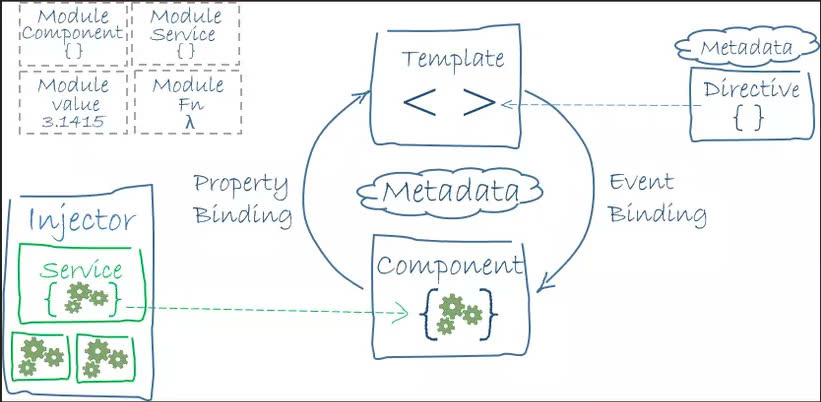
\includegraphics[width=0.8\textwidth]{latex/imgs/kientruc.jpg}
\caption{Kiến trúc tổng quan của ứng dụng Angular}
\end{figure}

\subsection{File package.json của dự án}

File \texttt{package.json} định nghĩa các dependencies và scripts của dự án:

\begin{lstlisting}[language=json]
{
  "name": "fron-end-spoify",
  "version": "0.0.0",
  "scripts": {
    "ng": "ng",
    "start": "ng serve",
    "build": "ng build",
    "watch": "ng build --watch --configuration development",
    "test": "ng test"
  },
  "private": true,
  "dependencies": {
    "@angular/animations": "^15.2.0",
    "@angular/cdk": "^15.2.9",
    "@angular/common": "^15.2.0",
    "@angular/compiler": "^15.2.0",
    "@angular/core": "^15.2.0",
    "@angular/forms": "^15.2.0",
    "@angular/material": "^15.2.9",
    "@angular/platform-browser": "^15.2.0",
    "@angular/platform-browser-dynamic": "^15.2.0",
    "@angular/router": "^15.2.0",
    "@fortawesome/fontawesome-svg-core": "^6.7.2",
    "@fortawesome/free-solid-svg-icons": "^6.7.2",
    "axios": "^1.8.4",
    "chart.js": "^4.4.9",
    "font-awesome": "^4.7.0",
    "rxjs": "~7.8.0",
    "tslib": "^2.3.0",
    "zone.js": "~0.12.0"
  },
  "devDependencies": {
    "@angular-devkit/build-angular": "^15.2.11",
    "@angular/cli": "~15.2.11",
    "@angular/compiler-cli": "^15.2.0",
    "@types/chart.js": "^2.9.41",
    "@types/jasmine": "~4.3.0",
    "autoprefixer": "^10.4.20",
    "jasmine-core": "~4.5.0",
    "karma": "~6.4.0",
    "karma-chrome-launcher": "~3.1.0",
    "karma-coverage": "~2.2.0",
    "karma-jasmine": "~5.1.0",
    "karma-jasmine-html-reporter": "~2.0.0",
    "postcss": "^8.5.3",
    "tailwindcss": "^3.4.17",
    "typescript": "~4.9.4"
  }
}
\end{lstlisting}

\subsection{Chạy ứng dụng trong môi trường phát triển}

Để khởi chạy ứng dụng trong môi trường phát triển:

\begin{lstlisting}[language=bash]
npm start
# hoặc
ng serve
\end{lstlisting}

Sau khi khởi chạy thành công, ứng dụng sẽ chạy tại địa chỉ \url{http://localhost:4200/}.

\subsection{Cấu hình TailwindCSS}

Dự án sử dụng TailwindCSS cho styling. File cấu hình \texttt{tailwind.config.js} được tạo tự động khi cài đặt TailwindCSS.

Nếu cần tùy chỉnh thêm, tạo file \texttt{tailwind.config.js} với nội dung sau:

\begin{lstlisting}[language=javascript]
/** @type {import('tailwindcss').Config} */
module.exports = {
  content: [
    "./src/**/*.{html,ts}",
  ],
  theme: {
    extend: {
      colors: {
        'spotify-green': '#1DB954',
        'spotify-black': '#191414',
      }
    },
  },
  plugins: [],
}
\end{lstlisting}

\subsection{Build ứng dụng cho môi trường production}

Để build ứng dụng cho môi trường production:

\begin{lstlisting}[language=bash]
npm run build
# hoặc
ng build --configuration production
\end{lstlisting}

Kết quả build sẽ được lưu trong thư mục \texttt{dist/}.

\subsection{Kiểm thử ứng dụng}

Dự án có sẵn các unit test và end-to-end test. Để chạy unit test:

\begin{lstlisting}[language=bash]
npm test
# hoặc
ng test
\end{lstlisting}

Kết quả test sẽ hiển thị trong terminal và trình duyệt.

\subsection{Xử lý sự cố thường gặp}

\begin{tcolorbox}[colback=red!5,colframe=red!40!black,title=Các lỗi thường gặp và cách khắc phục]
\begin{enumerate}
  \item \textbf{Lỗi "Node version not compatible"}:
  \begin{itemize}
    \item Cài đặt Node.js phiên bản tương thích (14.x - 16.x)
    \item Sử dụng công cụ quản lý phiên bản Node như NVM
  \end{itemize}
  
  \item \textbf{Lỗi khi cài đặt dependencies}:
  \begin{itemize}
    \item Xóa thư mục node_modules và file package-lock.json
    \item Chạy lại lệnh npm install
    \item Kiểm tra quyền truy cập hệ thống
  \end{itemize}
  
  \item \textbf{Lỗi Angular Material styles không load}:
  \begin{itemize}
    \item Kiểm tra imports trong file angular.json
    \item Thêm theme vào styles.scss
  \end{itemize}
\end{enumerate}
\end{tcolorbox}

\subsection{Tài liệu tham khảo}

\begin{itemize}
  \item Tài liệu Angular: \url{https://angular.io/docs}
  \item Tài liệu Angular Material: \url{https://material.angular.io/}
  \item Tài liệu TailwindCSS: \url{https://tailwindcss.com/docs}
  \item Tài liệu Chart.js: \url{https://www.chartjs.org/docs/latest/}
\end{itemize}
\end{xaiArtifact>

